%
% latex template for SAS documentation 
% name: sas.tex 
% date last modified: 16 mar 2018
% modified by: guru 
% 
%
\documentclass{article}

\usepackage{caption}
\usepackage[margin=1in]{geometry}
\usepackage{graphicx}
\usepackage{hyperref}
\usepackage{float}
\usepackage{tabularx}
\usepackage{titling}

\begin{document}

\title{
	
\includegraphics{images/um_logo.png} \\
	\vspace{0.1in}
	CSC431 \\
	\vspace{0.2in}
	\textbf{Download of Public-facing Data} \\
	\large System Architecture Specification \\
	Team \#3
}

\author{
	Jerry Bonnell
	\and Gururaj Shriram
	\and Re Chang
	\and Heyu Yao
	\and Lixiong Liang
}

\date{}
\maketitle

\clearpage
\section*{Version History}

\begin{tabularx}{\textwidth}{| l | l | X | l |}
	\hline
	\textbf{Version} & \textbf{Date} & \textbf{Author(s)} & \textbf{Change Comments} \\
	\hline
	1 & \today & Jerry Bonnell and Gururaj Shriram & First Draft \\
	\hline
\end{tabularx}

\clearpage
\tableofcontents

\clearpage
\listoffigures
\listoftables

\clearpage

\section{System Analysis}

\subsection{System Overview}

The System will be comprised of four main parts: a data manager, data packager, data converter, and data controller. The data manager will control the connection to the Access Database and handle database queries. The data packager will package all requested pieces of data into a compressed file if multiple pieces of data are requested. The data converter will convert files from the database into the users' desired file format from the list of supported file formats. The data controller will manage all of the other aspects of the system and manage the end-to-end pipeline of the downloading process. \\

The type of architecture used for the application is primarily the MVC (model view controller) style. The model service will sit in the Postgres database, Express will serve as the controller, and the view will be exist as part of another team's system.

\subsection{System Diagram}

\begin{figure}[h!]
	\begin{center}
		\caption{Download System Diagram}
		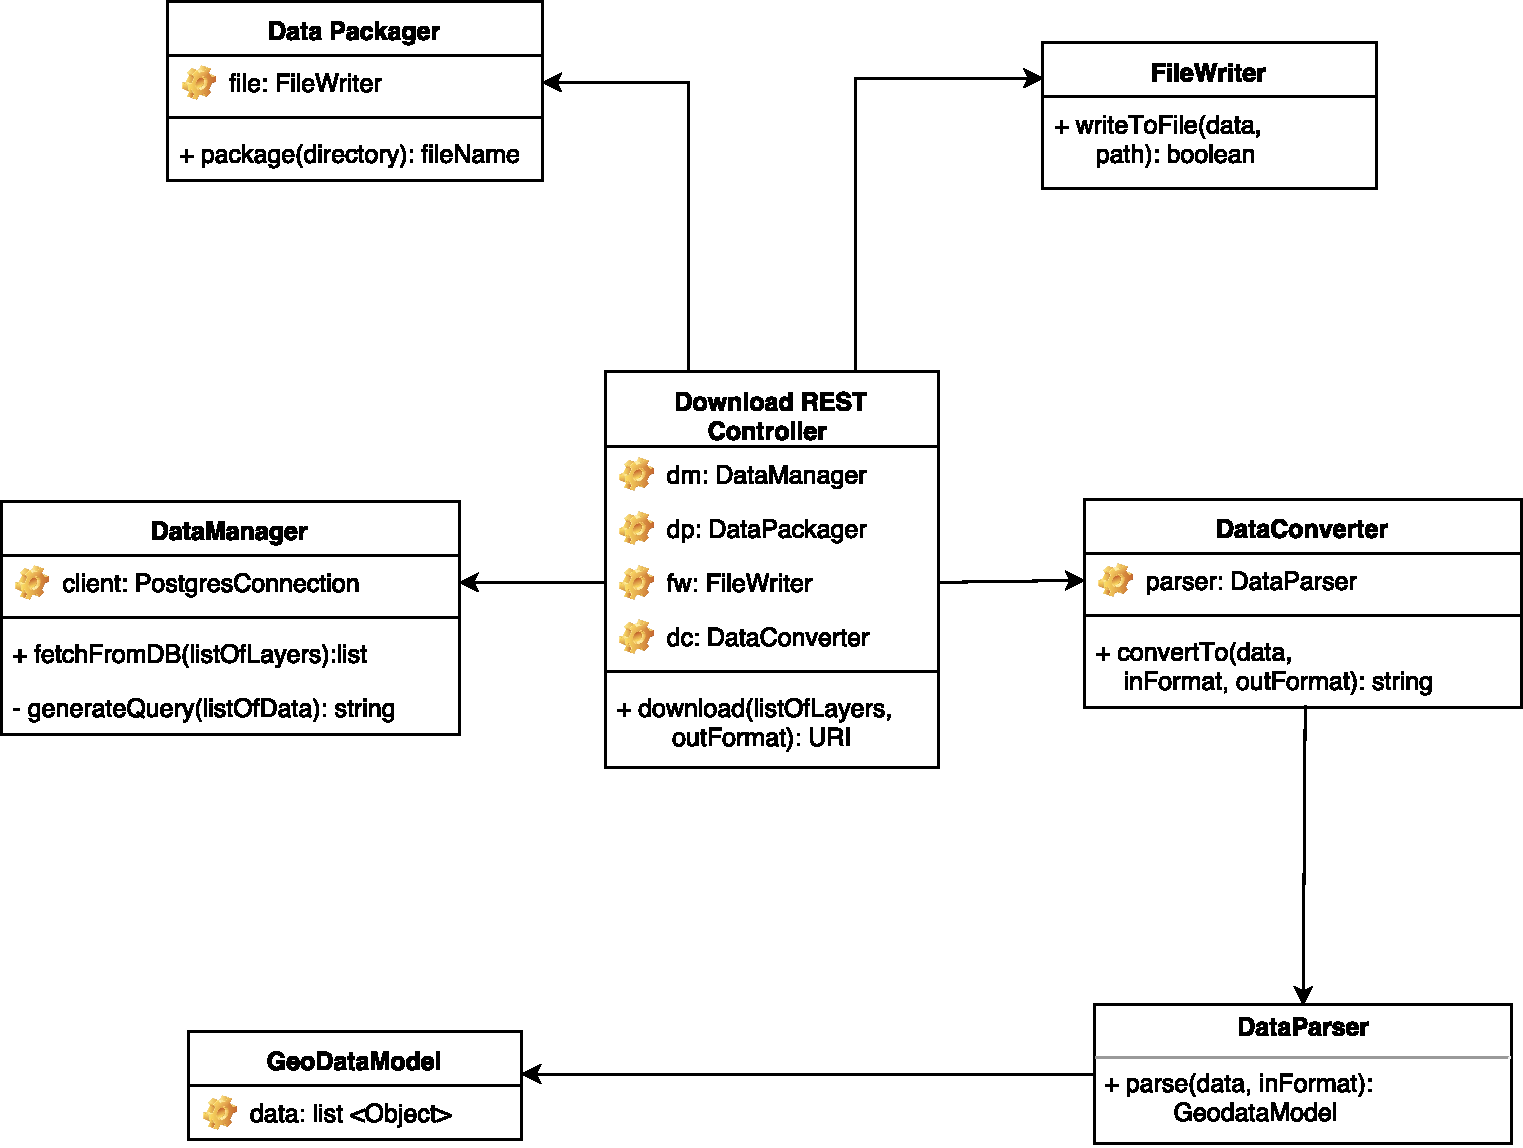
\includegraphics[width=\textwidth]{images/system_diagram.pdf}
	\end{center}
\end{figure}

\subsection{Actor Identification}

There are three types of human actors: unauthorized users, authorized users, and the administrators. Unauthorized users may only download public pieces of data unless they are granted permission to specific pieces of data from an administrator. Authorized users are allowed to download any piece of data. Administrators are able to download any piece of data as well as approve requests for unauthorized users to download private pieces of data. There are currently no plans for the system to support non-human actors, i.e. with an API. 

\subsection{Design Rationale}

\subsubsection{Architectural Style}

We will use the MVC, 3-tier architectural style pattern because this system is a web application which can be efficiently divided into to the model, view, and controller. The model lies on the database and manages the exchange of data. The controller receives user input, validates the input, and requests data download from the model. This system, which is part of a larger system, primarily lies on the backend and hence the "view" is only comprised of checkbox selections and download button requests from the user. 

\subsubsection{Design Pattern(s)}

Express is a flexible Node.js framework that provides a robust set of features. We predict that the following design patterns will be primarily used: \\

\begin{itemize} 
	\item Factory
	\item Singleton
	\item Middleware
	\item Stream
\end{itemize}


\subsubsection{Framework}

The web application will run on the \texttt{Node.js} JavaScript engine on the \texttt{Express} framework. \texttt{Express} allows for the successful implementation of a MVC on the backend and will facilitate a lightweight, efficient download pipeline. 

\textbf{Links:}
\begin{itemize} 
	\item \url{https://nodejs.org}
	\item \url{https://expressjs.com}
\end{itemize}

\clearpage

\section{Functional Design}

\begin{figure}[h!]
	\begin{center}
		\caption{Download Use Case}
		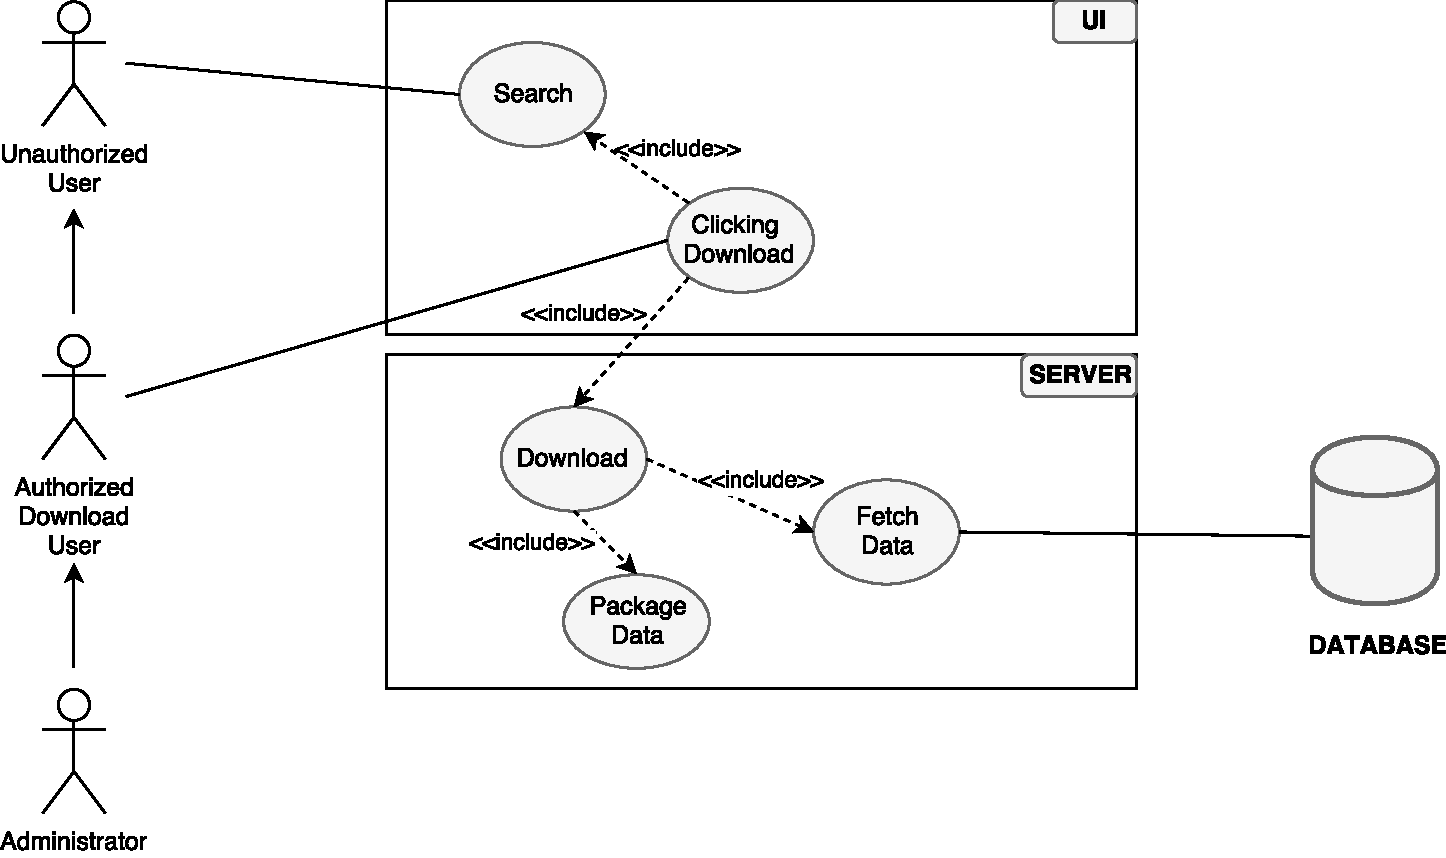
\includegraphics[width=\textwidth]{images/download_use_case.pdf}
	\end{center}
\end{figure}

\clearpage

\section{Structural Design}

Identify all components and model them using class diagrams.

\end{document}
